\scanpage{120}
$X$ schéma projectif

$M\subset K(X)$

\uline{Conditions équivalentes}

i) $\exists$ familles \uline{limitées} de faisceaux \inserted{loc. libres} $(F_i)(G_i)$ sur $X$, tel que $M$ contenu dans l'ens des
\[
\gamma(F_i)-\gamma(G_i)
\]

ii) $\exists$ un $n,N$ et une partie finie de \deleted{polynômes \unsure{P}} $\deleted{\unsure{P_1,P_i}}\ \Phi\subset Q[T]$, telle que les $x\in M$ soient de la forme $\gamma(F)-\gamma(G)$, $F$ et $G$ des quotients loc. libres de $\underline{O}(-n)^N$, de polynômes de Hilbert $\in\Phi$.

iii) \inserted{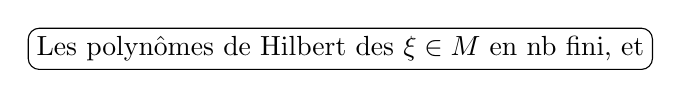
\begin{tikzpicture}\node[draw,rounded corners,inner sep=3pt] {Les polynômes de Hilbert des $\xi\in M$ \unsure{en nb fini, et}};\end{tikzpicture}}
$[\exists$ des faisceaux loc. libres, $A$ et $B$ ($\underline{O}(-n)^N$ si on veut) tels que les $\xi+\gamma(A)$ $(\xi\in M)$ soient décrits par des \uline{faisceaux} loc. libres, quotients de \deleted{un} \inserted{$B$.} \deleted{\unsure{un} faisceau $\underline{O}$ loc. libre ($\underline{O}(-n)^N$ si on veut}$]$.

$(\mathrm{iii})\Longrightarrow(\mathrm{ii})$ trivial, compte tenu que $A,B$ sont quotients de $\underline{O}(-n)^N$ pour $n,N$ convenables,

$(\mathrm{ii})\Longleftrightarrow(\mathrm{i})$ Par la caractérisation des familles limitées

$(\mathrm{ii})\Longrightarrow(\mathrm{iii})$ Car si $G=O(-n)^N/R$, on aura
\[
\xi=\gamma(F)-\gamma(\underline{O}(-n)^N)+\gamma(R)
\]
d'où
\[
\xi+\gamma(\underline{O}(-n)^N)=\gamma(F+R).
\]
Or $\deleted{F+}R$ est un quotient de $\unsure{\underline{O}(-n)^{N'}|\underline{O}(n)^{N'}}$, donc les $F+R$ \uuline{sont} \uline{quotients} d'un
\margin{119}
